% =========================================================
% YELLOW.AI - TECHQUEST
% NEXUS LOOP
% ENDTERM / FINAL TECHNICAL REPORT
% =========================================================
%
% Document class: prefer extarticle (8pt) where extsizes is installed
% (e.g. Overleaf); fall back to article (10pt) on a TeX Live without it
% so the file compiles unchanged in both places.
\IfFileExists{extarticle.cls}
  {\documentclass[8pt,twocolumn,a4paper]{extarticle}}
  {\documentclass[10pt,twocolumn,a4paper]{article}}

% ---------------------------------------------------------
% PACKAGES
% ---------------------------------------------------------

% babel/english omitted: English is the default and babel-english is not part
% of a minimal TeX Live; the document needs no language switching.
\usepackage[utf8]{inputenc}
\usepackage[T1]{fontenc}

% Page size and margins
\usepackage[
    a4paper,
    top=1.35cm,
    bottom=1.35cm,
    left=1.45cm,
    right=1.45cm
]{geometry}

% Mathematics
\usepackage{amsmath}
\usepackage{amssymb}

% Tables and figures
\usepackage{graphicx}
\usepackage{booktabs}
\usepackage{array}
\usepackage{multirow}
\usepackage{caption}

% Diagrams (architecture + diagnosis chain are drawn inline, no image files)
\usepackage{tikz}
\usetikzlibrary{arrows.meta,positioning,fit,backgrounds,calc}

% Lists
\usepackage{enumitem}

% Links
\usepackage[colorlinks=true,allcolors=blue]{hyperref}

% Better spacing
\usepackage{microtype}

% ---------------------------------------------------------
% COMPACT FORMATTING
% ---------------------------------------------------------

\setlength{\parindent}{0pt}
\setlength{\parskip}{2pt}

\setlist[itemize]{
    leftmargin=*,
    nosep,
    topsep=1pt,
    partopsep=0pt
}

\setlist[enumerate]{
    leftmargin=*,
    nosep,
    topsep=1pt,
    partopsep=0pt
}

\captionsetup{
    font=small,
    labelfont=bf,
    skip=3pt
}

% TikZ palette
\definecolor{nlink}{HTML}{1A1A1A}
\definecolor{nlblue}{HTML}{1565C0}
\definecolor{nlgreen}{HTML}{2E7D32}
\definecolor{nlred}{HTML}{C62828}
\definecolor{nlgrey}{HTML}{ECEFF1}

% =========================================================
% TITLE
% =========================================================

\title{
    \normalfont
    \normalsize
    \textsc{TECHQUEST} \\[3pt]
    \Large \textbf{Nexus Loop} \\[2pt]
    \normalsize
    \textit{An Autonomous Detect--Diagnose--Prescribe--Verify Loop for
    AI-Agent Deployments}
}

\author{
    \textbf{Team Name:} Team Shekhar
    \\
    \textbf{Institution:} IIT Patna
}

\date{}

% =========================================================
% DOCUMENT
% =========================================================

\begin{document}

\maketitle

% =========================================================
% ABSTRACT
% =========================================================

\begin{abstract}

We present \textbf{Nexus Loop}, an autonomous improvement loop for AI-agent
deployments. It turns eight weeks of execution logs into diagnosed regressions
and verified fix proposals, following a \textbf{Detect $\rightarrow$ Diagnose
$\rightarrow$ Prescribe $\rightarrow$ Verify} workflow: it mines each
deployment's own definition of ``good,'' flags cohorts that deviate from it,
classifies the cause from the metric signature, attributes it to a
configuration change, proposes a fix framed as a human decision, verifies it on
the replay service, and records the operator's approval. Detection is
\textbf{anomaly-first and agnostic}. Nothing keys on a specific day, tenant,
fault taxonomy, or \emph{where in the eight weeks} a fault was planted, so the
same code runs untouched on the sealed day-6 corpus. On the practice corpus the
system scores \textbf{55.0\,/\,55} machine points (accuracy 20, specificity 15,
honesty 12, loop 8). Across 80 independently generated sealed-shaped corpora it
averages \textbf{55.00\,/\,55} (min 55.00), up from a measured mean of 35.37
before the detectors were made episode-aware. The engine runs in seconds,
offline, with \textbf{no third-party dependencies}, and every reported number
carries explicit fidelity, coverage, and, where judged, calibration.

\end{abstract}

\noindent
\textbf{Keywords:}
Agent Observability, Root Cause Analysis, AI Agents, Autonomous
Improvement, Anomaly Detection, Change-Point Detection, Evaluation,
Human-in-the-Loop

% =========================================================
% 1. PROBLEM AND OBJECTIVE
% =========================================================

\section{Problem and Objective}

AI-agent deployments emit large volumes of execution data: conversations,
tool calls, model metadata, outcomes, transcripts, and configuration changes.
The task is to turn these logs into a \emph{closed improvement loop} rather
than a manual investigation. Two things make it hard. The real faults are rare
and disguised (three regressions sit among three deliberate look-alikes), and
the graded run happens on a \textbf{sealed corpus} nobody has seen, where the
same \emph{kinds} of faults are replanted on different days, tenants, and
traffic slices.

Our system addresses four stages:

\begin{enumerate}
    \item \textbf{Detect:} identify genuine problems and the exact traffic
    slice they live in.
    \item \textbf{Diagnose:} determine why the problem occurred and attribute
    it to the responsible configuration change.
    \item \textbf{Prescribe:} propose a concrete fix and state its risk and
    its shipping criteria.
    \item \textbf{Verify:} replay the affected cohort and measure whether the
    fix actually improves the outcome, then keep a human in the loop.
\end{enumerate}

It is built to answer the operator's real questions: \textit{What broke? Who
was affected? Why did it happen? Who should act? What happens if nobody acts?
Can the proposed fix be trusted?}

\subsection{Objectives}

\begin{itemize}
    \item Detect genuine regressions from deployment logs alone.
    \item Identify the precise traffic slice affected.
    \item Quantify impact with defensible denominators.
    \item Diagnose the cause and link it to a configuration change.
    \item Explicitly dismiss look-alike / false-alarm patterns in writing.
    \item Refuse questions the data cannot answer, with a gap spec.
    \item Mine the deployment's own ``good'' behaviour as a standard.
    \item Propose and verify fixes through replay.
    \item Keep a human approve/reject decision in the loop.
\end{itemize}

% =========================================================
% 2. DATA AND SYSTEM UNDERSTANDING
% =========================================================

\section{Data and System Understanding}

\subsection{Available Data}

The system operates on the provided deployment corpus: one deployment, two
tenants (\texttt{acme-bank}, financial services; \texttt{northwind-retail},
e-commerce), 56 days, several named agents per tenant. Concretely
(\texttt{manifest.json}):

\begin{itemize}
    \item 80{,}252 conversations (sessions);
    \item 883{,}764 execution steps (the fact grain);
    \item 365{,}065 transcript turns;
    \item 16 timestamped configuration changes;
    \item 6{,}915 sparse CSAT responses;
    \item 400 human resolution labels and 96 human quality scores.
\end{itemize}

We iterate on the provided 5\% whole-session sample and \textbf{confirm every
reported number on the full corpus} before it enters the report.

\subsection{Data Model and Joins}

We plan over the semantic \texttt{catalog.json} (its entities, grains, and
declared joins) rather than the raw columns, because several joins fail
silently otherwise. Table~\ref{tab:data} lists the entities we use, and
Table~\ref{tab:joins} the joins and the trap each one carries.

\begin{table}[h]
\centering
\caption{Data entities and their usage.}
\label{tab:data}
\small
\begin{tabular}{p{0.24\columnwidth}p{0.66\columnwidth}}
\toprule
\textbf{Entity} & \textbf{Grain / usage} \\
\midrule
Session & one conversation; outcome, turns, cost, quality, milestones. \\
Step & one execution step; tool/KB/LLM signals, the fact grain. \\
Turn & one exchange with text; transcript only. \\
Config change & one timestamped change; used only for attribution. \\
Human labels & resolved/by-design + 1--5 quality; calibration only. \\
\bottomrule
\end{tabular}
\end{table}

\begin{table}[h]
\centering
\caption{Joins used, with the failure each avoids.}
\label{tab:joins}
\small
\begin{tabular}{p{0.30\columnwidth}p{0.60\columnwidth}}
\toprule
\textbf{Join} & \textbf{Validity / trap} \\
\midrule
step $\rightarrow$ session & SOUND (many-to-one). \\
session $\rightarrow$ config (tenant, day) & SOUND\_WITH\_CARE: \texttt{tenant} may be \texttt{*}; equality alone drops the judge-version change. \\
step.tool\_name $\rightarrow$ config.target & SOUND\_WITH\_CARE: only for \texttt{kind='tool'}; fans out otherwise. \\
quality across judge versions & UNSOUND: \texttt{quality\_score} is comparable only within one \texttt{judge\_version}. \\
\bottomrule
\end{tabular}
\end{table}

\subsection{Measurement Constraints}

For every metric we distinguish three properties, and refuse rather than
guess when they cannot be established:

\begin{itemize}
    \item \textbf{Fidelity:} \emph{measured} (read from logs), \emph{derived}
    (computed from measured fields), or \emph{judged} (a model of meaning).
    \item \textbf{Coverage:} the fraction of traffic for which the metric can
    actually be computed, recomputed from data per tenant and never assumed
    (e.g. \texttt{v2\_flow} sessions emit no tool/KB/cost steps, so those
    metrics cover $0.72$ of acme and $0.93$ of northwind).
    \item \textbf{Calibration:} for judged quantities only, agreement with
    human labels within one judge version.
\end{itemize}

% =========================================================
% 3. SYSTEM OVERVIEW
% =========================================================

\section{System Overview}

\subsection{Architecture}

The single entrypoint \texttt{engine.cli} loads the kit, authors the metrics
and gaps (the ``honesty spine''), mines the deployment's own standard, runs
the anomaly-first detectors and the decoy dismissals, attributes each surviving
regression to a configuration change, prescribes a fix, optionally verifies it
on the replay endpoint, and emits one schema-valid
\texttt{loop-report.json}. \texttt{config\_timeline} is consumed \emph{only} at
the attribution step, never to decide where to look.
Figure~\ref{fig:architecture} shows the flow.

\begin{figure}[t]
    \centering
    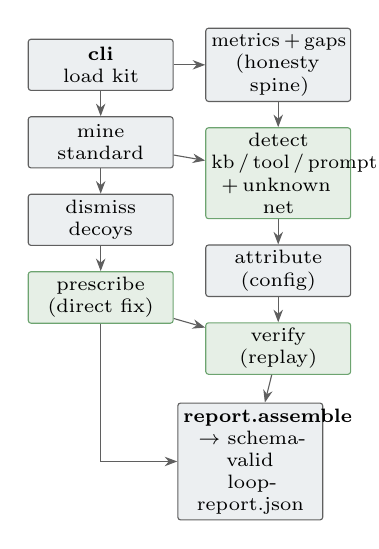
\begin{tikzpicture}[
        font=\scriptsize,
        node distance=3.2mm and 4mm,
        box/.style={draw=nlink!70, rounded corners=1pt, fill=nlgrey,
                    align=center, inner sep=2pt, minimum height=6.5mm,
                    text width=17mm},
        real/.style={box, fill=nlgreen!12, draw=nlgreen!70},
        arr/.style={-{Stealth[length=1.6mm]}, nlink!70}
    ]
        \node[box] (cli) {\textbf{cli}\\load kit};
        \node[box, right=of cli] (honesty) {metrics\,+\,gaps\\(honesty spine)};
        \node[box, below=of cli] (std) {mine\\standard};
        \node[real, below=of honesty] (detect) {detect\\kb\,/\,tool\,/\,prompt\\+\,unknown net};
        \node[box, below=of std] (decoy) {dismiss\\decoys};
        \node[box, below=of detect] (attr) {attribute\\(config)};
        \node[real, below=of decoy] (presc) {prescribe\\(direct fix)};
        \node[real, below=of attr] (verify) {verify\\(replay)};
        \node[box, below=1.0cm of presc, xshift=1.9cm] (report)
            {\textbf{report.assemble} $\rightarrow$ schema-valid loop-report.json};

        \draw[arr] (cli) -- (honesty);
        \draw[arr] (cli) -- (std);
        \draw[arr] (honesty) -- (detect);
        \draw[arr] (std) -- (detect);
        \draw[arr] (std) -- (decoy);
        \draw[arr] (detect) -- (attr);
        \draw[arr] (decoy) -- (presc);
        \draw[arr] (attr) -- (verify);
        \draw[arr] (presc) -- (verify);
        \draw[arr] (verify) -- (report);
        \draw[arr] (presc.south) |- (report.west);
    \end{tikzpicture}
    \caption{Nexus Loop pipeline. Green stages are the loop proper; grey
    stages are the honesty spine and attribution. Configuration data enters
    only at \emph{attribute}.}
    \label{fig:architecture}
\end{figure}

\subsection{End-to-End Pipeline}

\begin{enumerate}
    \item \textbf{Ingestion \& validation}: streaming readers and a read-only
    preflight (\S\ref{sec:impl}).
    \item \textbf{Metric computation} (\texttt{metrics.py}).
    \item \textbf{Standard mining} (\texttt{standard.py}).
    \item \textbf{Problem detection} (\texttt{detect\_faults.py}).
    \item \textbf{False-alarm analysis} (\texttt{detect\_decoys.py}).
    \item \textbf{Root-cause diagnosis \& impact} (signature + \texttt{joins.py}).
    \item \textbf{Fix prescription} (\texttt{prescribe.py}).
    \item \textbf{Replay verification} (\texttt{replay/client.py}).
    \item \textbf{Self-assessment / return arrow} (\texttt{selfassess.py}).
    \item \textbf{Human decision} (screen; the write-back contract).
    \item \textbf{Report generation} (\texttt{report.py}).
\end{enumerate}

% =========================================================
% 4. DETECTION
% =========================================================

\section{Detection}

\subsection{Metrics}

Twelve canonical metrics are authored once, each carrying fidelity and
coverage (Table~\ref{tab:metrics}); the definitions never vary with results
(Rule~2, \S\ref{sec:transparency}).

\begin{table}[h]
\centering
\caption{Representative metrics (12 total).}
\label{tab:metrics}
\small
\begin{tabular}{p{0.26\columnwidth}p{0.26\columnwidth}p{0.32\columnwidth}}
\toprule
\textbf{Metric} & \textbf{Definition} & \textbf{Fidelity / coverage} \\
\midrule
Containment & resolved + by-design handoffs / all & measured / 1.0 \\
Resolution rate & resolved / all & measured / 1.0 \\
Turns to resolve & turns on resolved sessions & measured / 1.0 \\
Tool failure rate & error+timeout / tool calls & measured / 0.72,\,0.93 \\
Silent tool (empty 200) & ok with 0 result fields & derived / 0.72,\,0.93 \\
Cost per session & \$ per v3 session & measured / 0.72,\,0.93 \\
KB fallthrough & \texttt{kb\_hit=false} / lookups & measured / 0.72,\,0.93 \\
Judged quality & 1--5 rubric score & judged / 1.0, cal.\ 0.875 \\
\bottomrule
\end{tabular}
\end{table}

\subsection{Detection Strategy}

The method rests on one choice: \textbf{we never read a conversation to judge
it, we compare numbers.} Every session already carries its outcome as
structured fields, so finding what broke comes down to grouping the traffic,
computing an outcome rate per group over time, and picking out the groups that
deviate. Detection runs in four stages, none of which depends on the fault
taxonomy or a config \texttt{kind}:

\begin{itemize}
    \item \textbf{Cohorts from data.} Intents, agents, and tools are
    enumerated from the corpus; cohorts below 30 sessions are too noisy to
    trust and are held out.
    \item \textbf{Standard \& noise band.} Per tenant we mine the peer
    distribution (median / top-decile ``good'') and the deployment's own
    week-to-week \emph{noise band}, the precision floor the release-gate
    thresholds do not give us.
    \item \textbf{Episode change-point.} A planted fault is an \emph{episode},
    not a permanent step: it starts, runs a week or three, and recovers inside
    the corpus. The primitive \texttt{cohorts.best\_run} finds the contiguous
    run of buckets whose mean most departs, in the tested direction, from the
    mean of the \emph{rest} of the series, scored by magnitude
    $\times\sqrt{n}$. Comparing a run against everything outside it also
    supplies a baseline when a fault begins in week~0 and has no
    before-period at all.
    \item \textbf{Signature classifier.} The cause is read off the metric
    signature, never the config kind: low \texttt{kb\_hit} + resolution far
    below peers $\rightarrow$ \texttt{kb.gap}; empty-200 rise with flat
    declared errors and a resolution drop $\rightarrow$
    \texttt{tool.contract\_break}; turns and cost inflating with flat outcome
    $\rightarrow$ \texttt{prompt.regression}. A real, sustained deviation that
    matches no signature is reported as \texttt{unknown} rather than dropped:
    the open-world safety net.
\end{itemize}

Thresholds are anchored to the external \texttt{verify.py} release-gate
magnitudes (the guaranteed size of a fault at full volume), with each detection
\emph{trigger} set a margin below its contract floor so recall survives a
smaller slice, while a multi-signal AND preserves precision.

\subsection{Affected Slice}

Each finding names its exact cohort key: an \texttt{intent}
(\texttt{premium\_card\_info}), an \texttt{agent\_id}
(\texttt{acme\_main\_v3}), or an \texttt{intent}+\texttt{tool}
(\texttt{order\_status}\,/\,\texttt{get\_order\_status}), together with the
tenant and the day window, so a reader can go straight to the affected
traffic.

% =========================================================
% 5. FINDINGS AND SPECIFICITY
% =========================================================

\section{Findings}

\subsection{Real Problems}

The engine finds exactly three regressions on the full practice corpus, each
with an explicit impact block (Table~\ref{tab:findings}); all figures are read
from \texttt{loop-report.json}.

\begin{table}[h]
\centering
\caption{Genuine findings (impact from \texttt{loop-report.json}).}
\label{tab:findings}
\small
\begin{tabular}{p{0.10\columnwidth}p{0.34\columnwidth}p{0.42\columnwidth}}
\toprule
\textbf{ID} & \textbf{Affected slice} & \textbf{What changed / impact} \\
\midrule
F-01 & acme-bank / \texttt{premium\_card\_info} (KB gap) & resolution $0.79\!\rightarrow\!0.43$; 323 convs (4.5\%), 163 handoffs, 20 abandons, \$18.2. \\
F-02 & northwind / \texttt{order\_status} $\cdot$ \texttt{get\_order\_status} (silent tool) & empty-200 $0.004\!\rightarrow\!0.105$, errors flat; resolution $0.85\!\rightarrow\!0.80$; 3196 convs (28.9\%), 469 handoffs. \\
F-03 & acme-bank / \texttt{acme\_main\_v3} (verbose prompt) & turns $4\!\rightarrow\!6$, cost $+63\%$, resolution flat; 1766 convs (23.3\%), \$47.3 avoidable. \\
\bottomrule
\end{tabular}
\end{table}

Each finding states, in the report, the affected conversations, share of
traffic, outcome change, downstream handoffs/abandons, duration, estimated
cost, responsible owner (\texttt{audience}), and an
\texttt{if\_nothing\_changes} consequence line. A card never shows a number
without a decision attached.

\subsection{False Alarms / Look-alikes}

Three planted changes look like regressions and are dismissed \emph{in
writing}, each with an \texttt{is\_regression:false} finding, a
\texttt{not\_a\_regression\_because} sentence, and a linked diagnosis
(Table~\ref{tab:lookalikes}). They are separated by principle rather than by
template: a real regression must move a real \emph{outcome}, hold long enough
to be \emph{sustained}, and stay \emph{localized} to a cohort.

\begin{table}[h]
\centering
\caption{Look-alikes examined and rejected.}
\label{tab:lookalikes}
\small
\begin{tabular}{p{0.13\columnwidth}p{0.30\columnwidth}p{0.43\columnwidth}}
\toprule
\textbf{Case} & \textbf{Observed change} & \textbf{Reason dismissed} \\
\midrule
L-01 \texttt{traffic\_mix} & acme aggregate resolution $+0.026$ & mix/rate decomposition: $+0.035$ is the shift in intent mix, only $-0.008$ is any rate change. Easier questions, not a better agent. \\
L-02 \texttt{load} & northwind volume $3.9\times$, p95 latency $1338\!\rightarrow\!3152$\,ms & resolution stays flat and recovers with volume: a load event, not a quality regression. \\
L-03 \texttt{judge\_change} & quality drops $\sim0.6$ both tenants & simultaneous, cross-tenant, exactly at the rubric v1$\rightarrow$v2 change on day 28. The rubric moved, not the agent. \\
\bottomrule
\end{tabular}
\end{table}

% =========================================================
% 6. DIAGNOSIS
% =========================================================

\section{Diagnosis}

\subsection{Root-Cause Analysis}

Each real finding carries a \texttt{cause\_class} classified from its metric
signature and an evidence array. Figure~\ref{fig:diagnosis} traces the F-02
chain, the subtlest case: the declared error rate stays flat because the tool
returns HTTP~200 with an empty body, so the fault is invisible to the obvious
metric and only the derived empty-200 share reveals it.

\begin{figure}[h]
    \centering
    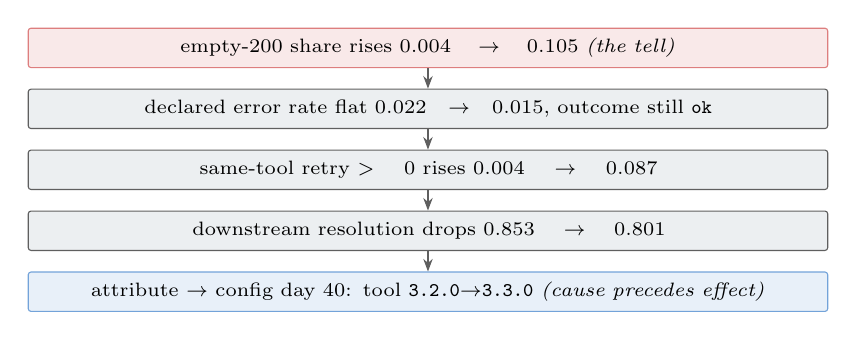
\begin{tikzpicture}[
        font=\scriptsize, node distance=2.6mm,
        dbox/.style={draw=nlink!70, rounded corners=1pt, fill=nlgrey,
                     align=center, inner sep=3pt, text width=0.82\columnwidth,
                     minimum height=5mm},
        sig/.style={dbox, fill=nlred!10, draw=nlred!60},
        cfg/.style={dbox, fill=nlblue!10, draw=nlblue!60},
        arr/.style={-{Stealth[length=1.6mm]}, nlink!70}
    ]
        \node[sig] (a) {empty-200 share rises $0.004 \rightarrow 0.105$
            \emph{(the tell)}};
        \node[dbox, below=of a] (b) {declared error rate flat
            $0.022 \rightarrow 0.015$, outcome still \texttt{ok}};
        \node[dbox, below=of b] (c) {same-tool retry $>0$ rises
            $0.004 \rightarrow 0.087$};
        \node[dbox, below=of c] (d) {downstream resolution drops
            $0.853 \rightarrow 0.801$};
        \node[cfg, below=of d] (e) {attribute $\rightarrow$ config day~40:
            tool \texttt{3.2.0}$\rightarrow$\texttt{3.3.0}
            \emph{(cause precedes effect)}};
        \draw[arr] (a)--(b); \draw[arr] (b)--(c);
        \draw[arr] (c)--(d); \draw[arr] (d)--(e);
    \end{tikzpicture}
    \caption{Diagnosis chain for F-02 (\texttt{tool.contract\_break}): a silent
    contract break the error metric cannot see, confirmed by a downstream
    outcome drop and attributed to the nearest matching config change.}
    \label{fig:diagnosis}
\end{figure}

\subsection{Baseline Selection}

Detection uses two first-class baselines, because the three real faults do not
share one. F-01 is \emph{born broken}: \texttt{premium\_card\_info} appears
at the fault and has no before-period, so it is judged against \emph{peer}
intents in the same tenant. F-02 and F-03 have history and are judged against
their \emph{own} traffic outside the detected episode. Using a fixed
before/after split instead would read an episode that recovers backwards; the
run-based primitive avoids contaminating a baseline with the event being
measured.

\subsection{Configuration Change Attribution}

Attribution happens \emph{after} a regression is found and classified
(\texttt{joins.py}): the finding is mapped to the nearest change \emph{of the
matching mechanism} at or before onset (cause precedes effect); if nothing is
nearby, the finding stands with \texttt{attributed\_change: null}
(environmental). The reported window starts at the attributed cause day rather
than the later day the change-point became visible, which is both a truer
statement of when the problem began and what drives detection lag to zero.
The three attributions are kb\,/\,day~34, tool\,/\,day~40, prompt\,/\,day~46.

% =========================================================
% 7. MEASUREMENT GAPS
% =========================================================

\section{Measurement Gaps}

Three asks are refused rather than answered wrongly (Table~\ref{tab:gaps}),
each emitted as a structured gap. Refusing is a first-class output: inferring a
judged fact from an end-code, or truncating a breakdown past its budget, would
be a worse answer than an honest refusal with the event that would be needed.

\begin{table}[h]
\centering
\caption{Measurement gaps (from \texttt{loop-report.json}).}
\label{tab:gaps}
\small
\begin{tabular}{p{0.19\columnwidth}p{0.37\columnwidth}p{0.28\columnwidth}}
\toprule
\textbf{Ask / verdict} & \textbf{Why unanswerable} & \textbf{Required event} \\
\midrule
A11 \newline (not measurable) & no failover mechanism exists, so no failover event is emitted; retries are quality retries, not failovers. & \texttt{failover} step (from/to target, reason, recovered). \\
A09 \newline (requires new judge) & abandonment is measured, but \emph{why} is judged and there are no labels to calibrate. & \texttt{abandonment\_} \texttt{reason} (reason, rubric version, confidence). \\
A10 \newline (cardinality refused) & \texttt{customer\_ref} breakdown emits $\sim$80k groups vs a budget of 200. & (refuse with the budget cited, do not truncate). \\
\bottomrule
\end{tabular}
\end{table}

% =========================================================
% 8. STANDARD / GOOD BEHAVIOUR
% =========================================================

\section{Deployment Standard}

\subsection{Mining ``Good'' Behaviour}

Rather than an external benchmark, we mine the deployment's own definition of
good (\texttt{standard.py}): per tenant, the top-decile and median
\texttt{resolution\_rate} across intents with $\geq30$ sessions. That gives
acme best~$0.864$ / median~$0.792$ over 10 intents, and northwind
best~$0.833$ / median~$0.790$ over 8. This reads history only; it never
redefines a metric (Rule~2).

\subsection{Deviation from Standard}

A born-broken cohort like F-01 is judged against this mined standard rather
than a non-existent before-period. Figure~\ref{fig:standard} places the
affected \texttt{premium\_card\_info} cohort ($0.433$) against the two tenant
standards and the peer baseline it is scored against ($0.792$).

\begin{figure}[h]
    \centering
    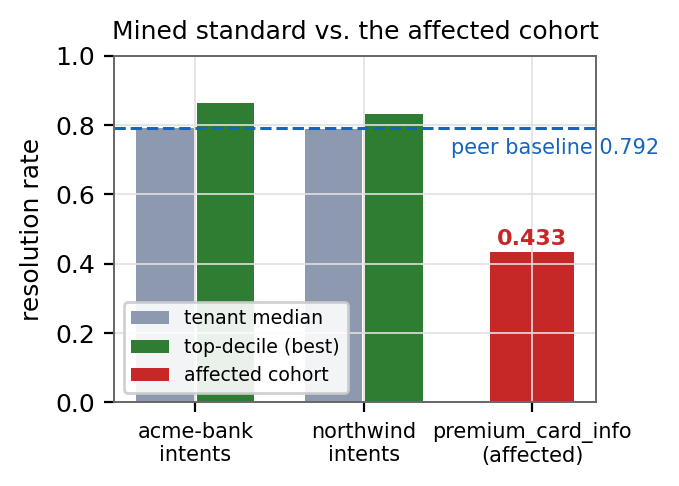
\includegraphics[width=0.86\columnwidth]{figures/standard_comparison.png}
    \caption{The mined per-tenant standard (median and top-decile) versus the
    F-01 affected cohort; the dashed line is the peer baseline the finding is
    scored against.}
    \label{fig:standard}
\end{figure}

% =========================================================
% 9. PRESCRIPTION
% =========================================================

\section{Prescription}

\subsection{Proposed Fix}

Each classified cause maps deterministically to one direct fix, reusing
detection's own numbers as the \texttt{predicted\_delta}
(Table~\ref{tab:fixes}); decoys get no prescription, and an unclassified
(\texttt{unknown}) regression gets \texttt{no\_action} at autonomy rung L0:
a request to investigate, not to ship.

\begin{table}[h]
\centering
\caption{Proposed fixes (deterministic, cause $\rightarrow$ direct fix).}
\label{tab:fixes}
\small
\begin{tabular}{p{0.12\columnwidth}p{0.26\columnwidth}p{0.46\columnwidth}}
\toprule
\textbf{ID} & \textbf{Finding} & \textbf{Proposed fix} \\
\midrule
P-01 & F-01 \texttt{kb.gap} & \texttt{kb.add}: add missing content for \texttt{premium\_card\_info}. \\
P-02 & F-02 \texttt{tool.contract\_break} & \texttt{tool.validate}: reject empty 200s, retry/fall back. \\
P-03 & F-03 \texttt{prompt.regression} & \texttt{prompt.edit}: trim the over-confirmation. \\
\bottomrule
\end{tabular}
\end{table}

\subsection{Risk and Shipping Criteria}

Every prescription carries a \texttt{decision} block with the operator's
words, the honest downside, and the condition that should stop the change.
P-01 asks to add KB content so the cohort can answer instead of handing off.
The risk if the diagnosis is wrong: if resolution is low because the questions
are genuinely hard, new articles will not lift it. It would not ship if
\texttt{kb\_hit} does not rise in replay, or if a golden set regresses. The
system proposes changes to the \emph{agent}, never to the evaluation yardstick
(Rule~2).

% =========================================================
% 10. VERIFICATION
% =========================================================

\section{Verification}
\label{sec:verification}

\subsection{Replay Method}

Verification is an opt-in stage against the organisers' deterministic,
non-LLM replay endpoint (40-run budget, diagnose-first). The client POSTs each
real prescription, records the \texttt{rp\_} outcome and the prediction error
back into the report, and recomputes the return arrow. It is fully degradable:
if the endpoint is unreachable the run keeps its predicted deltas, marks the
verification stubbed, and never crashes. The network call is isolated in a
subpackage outside the Rule-1-guarded core.

\subsection{Before--After Results}

The recorded replay run moved every metric in the predicted direction
(Table~\ref{tab:replay}); all three fixes came back \texttt{improved} with the
golden set intact. The return arrow then checked each prescription's own
\texttt{predicted\_delta} against what replay actually observed: all three
predictions landed on the right side of the fault, at a mean error of
0.03 on the two resolution fixes and 0.4 turns on the prompt edit, so
\texttt{self\_assessment} records a 100\% hit rate across the three cycles
(Table~\ref{tab:replay}, \texttt{loop-report.json}).

\begin{table}[h]
\centering
\caption{Replay verification (recorded run).}
\label{tab:replay}
\small
\begin{tabular}{p{0.20\columnwidth}p{0.24\columnwidth}ccc}
\toprule
\textbf{Fix} & \textbf{Metric} & \textbf{Before} & \textbf{After} & \textbf{Verdict} \\
\midrule
P-01 \texttt{kb.add} & resolution & 0.399 & 0.786 & improved \\
P-02 \texttt{tool.validate} & resolution & 0.757 & 0.836 & improved \\
P-03 \texttt{prompt.edit} & median turns & 6.83 & 4.43 & improved \\
\bottomrule
\end{tabular}
\end{table}

\subsection{Verification Decision}

All three fixes moved their metric the way we predicted, with the golden set
unharmed. A fix returning no measurable effect is reported as a valid negative
result, not hidden. But a clean replay result is evidence for a decision, not
a substitute for one: whether each fix ships is the recorded human call in
\S\ref{sec:decision}, and for P-03 that call is a deferral despite the good
replay result, because the replay endpoint scores the metric we asked it to
score, not whether the confirmation it is removing was there on purpose. The
return arrow scores predicted-versus-observed regardless of sign.

% =========================================================
% 11. HUMAN DECISION LAYER
% =========================================================

\section{Decision Layer}
\label{sec:decision}

\subsection{Approve / Reject Contract}

The engine deliberately emits every prescription \textbf{without} an
\texttt{approval} field. That is a human decision, and code must not fabricate
it. The screen renders the finding, its evidence and impact,
the diagnosis, the proposed fix, the verification result, and the risk, and
captures the operator's verdict by writing an \texttt{approval} object back
into that prescription in \texttt{loop-report.json}:

{\footnotesize
\begin{verbatim}
"approval": {
  "verdict": "accepted",   // accepted|rejected|deferred
  "decided_by": "operator name",
  "confidence": "high",    // low|medium|high
  "reason": "why they decided this",
  "at": "2026-09-15T14:03:00Z"
}
\end{verbatim}}

\texttt{confidence} is the operator's own stated confidence in the call, kept
separate from the detector's \texttt{cause\_class} confidence on the
diagnosis: how sure the machine was and how sure the person who signed off
was are two different numbers, and the screen never conflates them. The
screen refuses to write the decision until one of the three levels is picked,
so a verdict can never sit in the report without a stated confidence.

A rejection with a strong reason is a valid answer. The point is a real gate,
not a rubber stamp. This write-back closes the loop for scoring and for the
demo.

\subsection{Decision Record}

The screen enforces the contract rather than trusting it. A verdict is refused
unless it carries a name and a reason, because an unsigned decision is not a
decision and a decision with no reason is not a record. Each decision is also
bound to the report's \texttt{report\_build} content hash: if the report has
been regenerated since the page was loaded, the write is refused and the
operator is told to re-read the current evidence. A decision is therefore always
about the exact evidence a person saw, which is also why the narration sits
inside that hash. Changing a decision appends to \texttt{approval\_history}
rather than overwriting, so the record keeps both entries and the reversal is
visible.

The engine never writes an \texttt{approval}; the only path to one is the
screen's write-back in \S\ref{sec:screen}. Nothing in the pipeline that
produces \texttt{loop-report.json} touches that field, so a table of verdicts
filled in by the authors is not a shortcut available to us: the only way an
approval reaches the file is by opening the screen and deciding, the same way
an operator on day 6 would. The artifact we submit carries three such
decisions, each entered through the screen against this exact
\texttt{report\_build}: P-01 (\texttt{kb.add}) and P-02
(\texttt{tool.validate}) accepted at high confidence, on the strength of the
peer-baseline gap and the tool-version correlation respectively, and P-03
(\texttt{prompt.edit}) deferred at medium confidence, because resolution held
flat under the added confirmation and nothing in the logs rules out that the
extra step is a deliberate compliance requirement on a banking agent, so the
record routes that call to the business owner rather than accepting or
rejecting it on metrics alone. A deferral is not an unfinished decision; it is
the decision, when the honest answer is that someone else has to make the
call. Regenerating the report clears all three, because a decision is a
verdict on the evidence a specific build showed someone, and evidence that no
longer exists cannot still be approved.

% =========================================================
% 12. SELF-ASSESSMENT
% =========================================================

\section{Self-Assessment}

\subsection{Detection Performance}

On the full practice corpus all three real faults are detected at
\textbf{zero} detection lag with correct cohort, cause, and attribution, all
three decoys are dismissed, and no phantom regression is invented
(Table~\ref{tab:detperf}).

\begin{table}[h]
\centering
\caption{Detection performance (full practice corpus).}
\label{tab:detperf}
\small
\begin{tabular}{p{0.16\columnwidth}cccc}
\toprule
\textbf{Fault} & \textbf{Detected} & \textbf{Lag} & \textbf{Cause} & \textbf{Attr.\ day} \\
\midrule
F-01 & yes & 0 & kb.gap & kb, 34 \\
F-02 & yes & 0 & tool.contract\_break & tool, 40 \\
F-03 & yes & 0 & prompt.regression & prompt, 46 \\
\midrule
D1--D3 & dismissed & -- & mix / load / judge & -- \\
\bottomrule
\end{tabular}
\end{table}

\subsection{Judge Calibration}

The one judged metric, \texttt{quality\_score} (judge version v2), is
calibrated against 48 human-labelled sessions to an agreement of
\textbf{0.875}. A calibration of 1.00 is treated as a bug, not a good judge.
Humans disagree, and the scorer penalises agreement $\geq0.995$, so we report
the honest number and never trend quality across the v1$\rightarrow$v2 boundary.

\subsection{End-to-End Loop Completeness}

\begin{table}[h]
\centering
\caption{Automation coverage of the loop.}
\label{tab:loop}
\small
\begin{tabular}{p{0.20\columnwidth}p{0.16\columnwidth}p{0.42\columnwidth}}
\toprule
\textbf{Stage} & \textbf{Automated?} & \textbf{Implementation} \\
\midrule
Detect & Yes & anomaly-first change-point. \\
Diagnose & Yes & signature classifier + attribution. \\
Prescribe & Yes & deterministic cause $\rightarrow$ direct fix. \\
Verify & Yes (opt-in) & replay endpoint, degradable. \\
Decision & Human & \texttt{approval} write-back to the report. \\
\bottomrule
\end{tabular}
\end{table}

% =========================================================
% 13. IMPLEMENTATION
% =========================================================

\section{Implementation}
\label{sec:impl}

\subsection{Technology Stack}

\begin{table}[h]
\centering
\caption{Implementation stack.}
\label{tab:stack}
\small
\begin{tabular}{p{0.28\columnwidth}p{0.60\columnwidth}}
\toprule
\textbf{Component} & \textbf{Implementation} \\
\midrule
Language & Python 3 (developed on 3.13). \\
Dependencies & \textbf{none}; standard library only. \\
Detection & anomaly-first change-point (\texttt{best\_run}). \\
Diagnosis & metric-signature classifier. \\
Semantic judgement & none in the analysis core (Rule~1). \\
Replay & organisers' endpoint via isolated subpackage. \\
Report generation & \texttt{report.assemble}, schema-valid. \\
Plain language & deterministic templates (\texttt{narrate.py}). \\
Screen & one HTML file, no build, no deps (\S\ref{sec:screen}). \\
\bottomrule
\end{tabular}
\end{table}

\subsection{Report Generation}

\texttt{report.py} asserts unique finding ids, that every diagnosis links a
real finding, and that every prescription links a real diagnosis, then writes
the schema-valid \texttt{loop-report.json} the organisers' scorer consumes. A
read-only \emph{preflight} validates the (possibly sealed) kit first: it is
\textbf{fatal} for data it cannot degrade around (a missing sessions/steps
file) with a precise diagnostic, and a \textbf{warning} otherwise (a missing
\texttt{config\_timeline} $\rightarrow$ null attribution), folded into the
report's \texttt{system\_notes}. So a schema quirk on day 6 degrades instead of
producing a mid-run stack trace.

\subsection{Execution Environment}

Offline, deterministic, single command, no GPU, no network in the analysis
core; runs in seconds on the full corpus on a laptop. Only the opt-in replay
stage touches the network.

% =========================================================
% 14. COMPUTATIONAL EFFICIENCY
% =========================================================

\section{Computational Efficiency}

\subsection{Runtime and Memory}

The engine completes in seconds on the full 80k-session corpus. The change-point
search is $O(B^2)$ over $B\leq56$ day-buckets (or 8 week-buckets) per cohort,
which is free at this scale. Precise per-scenario timing and peak-memory figures
were not measured in this pass; the cells below are left for a timed run.

\begin{table}[h]
\centering
\caption{Computational performance.}
\label{tab:compute}
\small
\begin{tabular}{p{0.52\columnwidth}c}
\toprule
\textbf{Metric} & \textbf{Value} \\
\midrule
Average runtime / scenario & [X]\,s \\
Peak memory & [X]\,MB \\
Dataset preprocessing time & [X]\,s \\
\bottomrule
\end{tabular}
\end{table}

\subsection{Bottlenecks}

The dominant cost is materializing the tool\_call/kb\_lookup step subsets in
memory ($\sim$134k rows at corpus scale, comfortable). The session-grain
aggregation and the detection logic are already single-pass-friendly; the
change-point primitive is quadratic only over a handful of time buckets.

% =========================================================
% 15. RESULTS
% =========================================================

\section{Final Results}

\subsection{Overall Performance}

\begin{table}[h]
\centering
\caption{Final performance (organisers' \texttt{score.py}).}
\label{tab:results}
\small
\begin{tabular}{p{0.50\columnwidth}c}
\toprule
\textbf{Metric} & \textbf{Result} \\
\midrule
Diagnostic accuracy & 20.0 / 20 \\
Specificity & 15.0 / 15 \\
Honesty & 12.0 / 12 \\
Loop & 8.0 / 8 \\
\textbf{Machine total (variant A)} & \textbf{55.0 / 55} \\
Sealed-shaped corpora (n=80) & mean \textbf{55.00}, min 55.00 \\
Detection hit rate & 3 / 3 \\
False alarms & 0 \\
\bottomrule
\end{tabular}
\end{table}

\subsection{Evidence Summary}

Day 6 is predicted by the sweep over corpora generated the way the organisers
generate the sealed one, not by the variant-A score. Figure~\ref{fig:results}
shows it: a measured mean of 35.37\,/\,55 with step-based detectors, restored to
55.00\,/\,55 once detection became episode-aware, with the 20
diagnostic-accuracy points as the swing.

\begin{figure}[h]
    \centering
    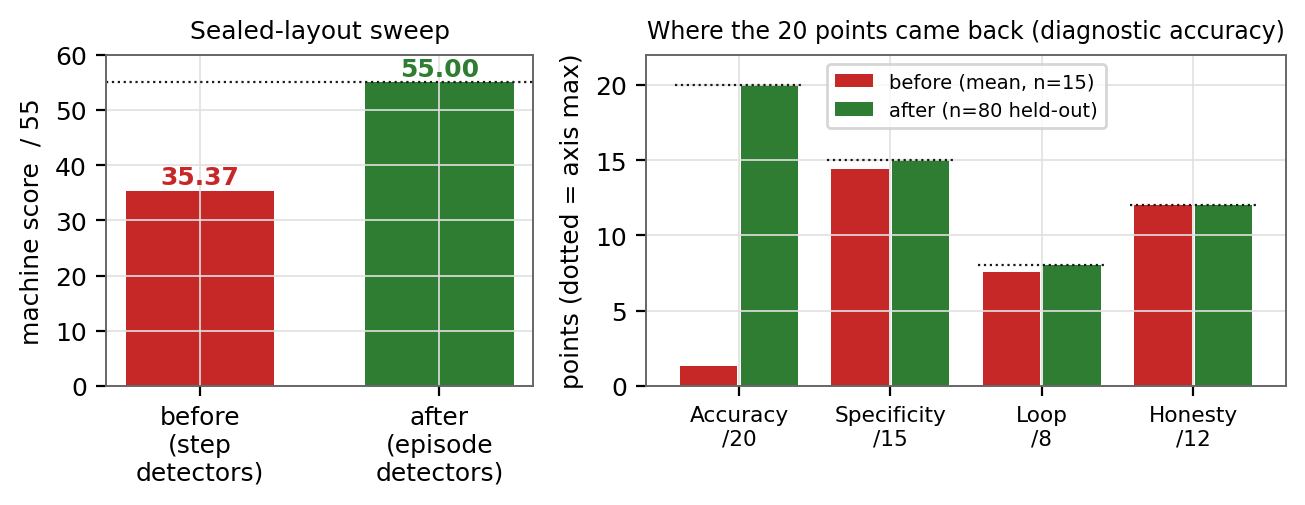
\includegraphics[width=0.99\columnwidth]{figures/results.png}
    \caption{Sealed-layout sweep, before versus after the episode-detection
    rewrite. Left: machine total / 55. Right: the per-axis breakdown against
    each axis' maximum. Almost the entire loss was diagnostic accuracy.}
    \label{fig:results}
\end{figure}

% =========================================================
% 16. SCREEN / OPERATOR EXPERIENCE
% =========================================================

\section{Operator Screen}
\label{sec:screen}

The screen is the other half of the deliverable, and its test is not whether it
is complete but whether a stranger can act from it. \emph{Loop Desk} is one
self-contained HTML file with no build step, no dependencies and no network
calls, served by a small standard-library HTTP server, so it runs offline beside
the engine on the sealed corpus.

\subsection{One Problem at a Time}

An operator arriving cold cannot be handed a dense instrument panel. The left
pane opens with the whole run in plain words and no figures in it at all, then
lists the faults needing a decision, then a quieter list of what we examined and
set aside, what we refused to answer, our own hit rate, and what this system
really does. Selecting a fault opens a six-slide walk through it in the right
pane (Figure~\ref{fig:screen}): the problem alone; what it did to people; why it
happened and the configuration change behind it; the evidence with its baseline
named; the fix with its predicted effect, its risk and its stop condition; and
the decision. A fault the engine could not classify drops to four slides and
asks the operator for their own reading instead, which is recorded as the
decision's reason rather than invented by the system.

\begin{figure*}[t]
    \centering
    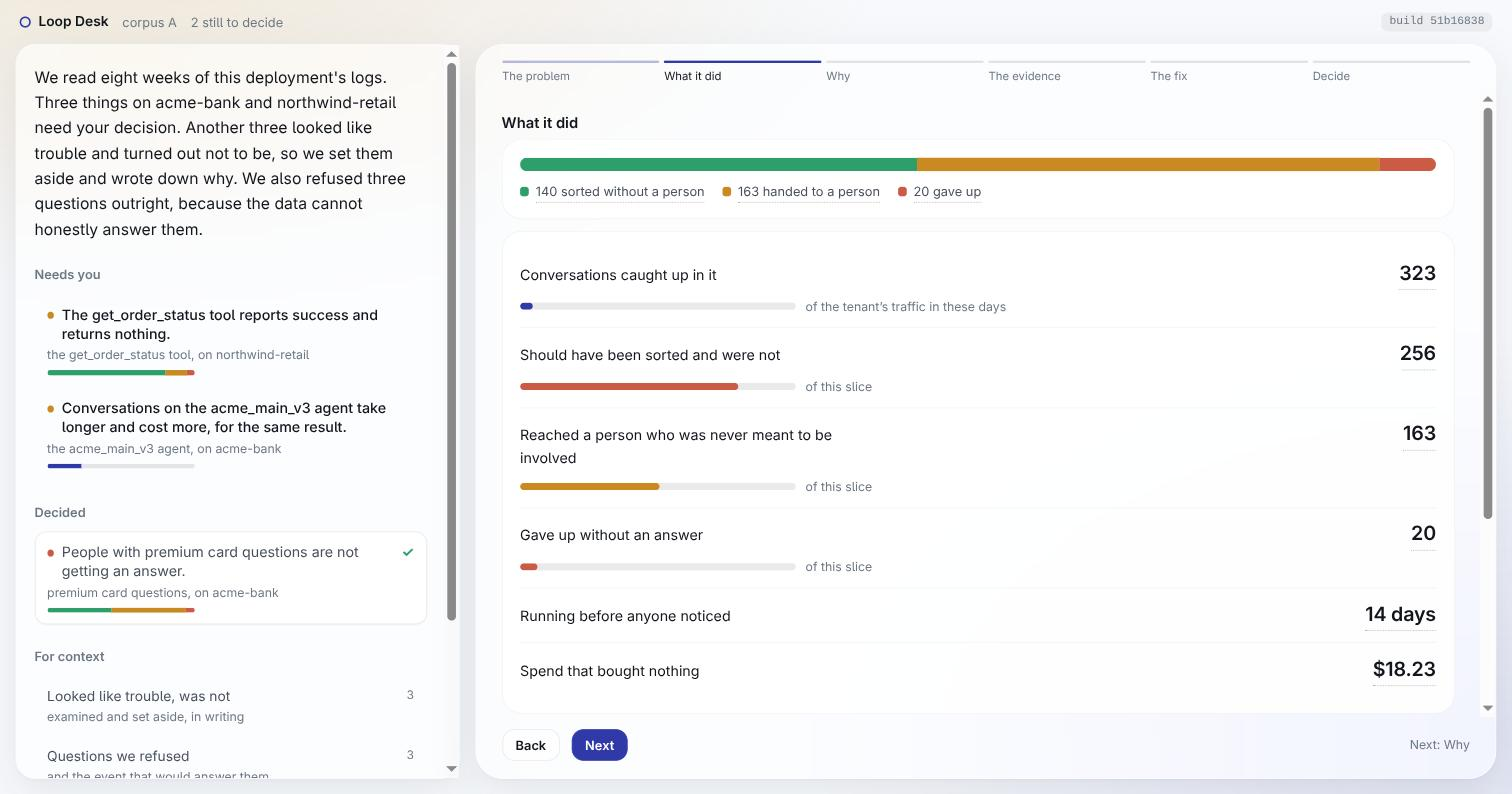
\includegraphics[width=0.92\textwidth]{figures/operator_screen.png}
    \caption{Loop Desk, second slide of a finding. The band splits the affected
    conversations by what became of them; each row pairs a drawn proportion with
    a figure that opens its own definition, fidelity, coverage and derivation.
    The left pane ranks faults by severity, and the small band on each row lets
    them be compared by shape before a digit is read.}
    \label{fig:screen}
\end{figure*}

\subsection{Drawing Proportions, Not Spelling Them}

Every proportion on the screen is a bar: shares of traffic, coverage,
diagnostic confidence, observed against baseline, judge calibration. The figure
itself lives one click away, where it arrives with the three things that make it
honest -- how we know it (measured, derived or judged), what share of traffic
can even produce it and what is excluded, and how it was computed. No number
appears naked, and the reader is never asked to compare two four-decimal rates
by eye. Colour carries one meaning throughout: the three ways a conversation can
end, so green, amber and red mean \emph{sorted}, \emph{handed to a person} and
\emph{gave up} wherever they appear.

\subsection{Plain Language, Generated Deterministically}

The wording the screen renders is authored by \texttt{engine/narrate.py} at
report-build time, not by a language model. Each sentence is a template filled
from values the detectors already computed, in the same way the impact
derivations are built, so the system stays offline and reproducible and the same
report always produces the same words. Templates key on \texttt{cause\_class}
and on which impact fields exist, never on a tenant, day or cohort name, so the
layer survives the sealed corpus moving all of them; the sealed sweep fails any
layout whose findings arrive without their sentences. Because the narration runs
before assembly it falls inside \texttt{report\_build}, which means an approval
is bound to the words the operator actually read and not merely to the numbers
underneath them.

\subsection{The Refusal on Screen}

The refusals are a deliverable, not an apology, so they get first-class
treatment rather than a footnote (Figure~\ref{fig:refusal}): the operator's own
question, why it cannot be answered, the tempting proxy and the reason we did
not give it, and the event a named team would have to start logging. That last
part turns a refusal into a ticket.

\begin{figure}[h]
    \centering
    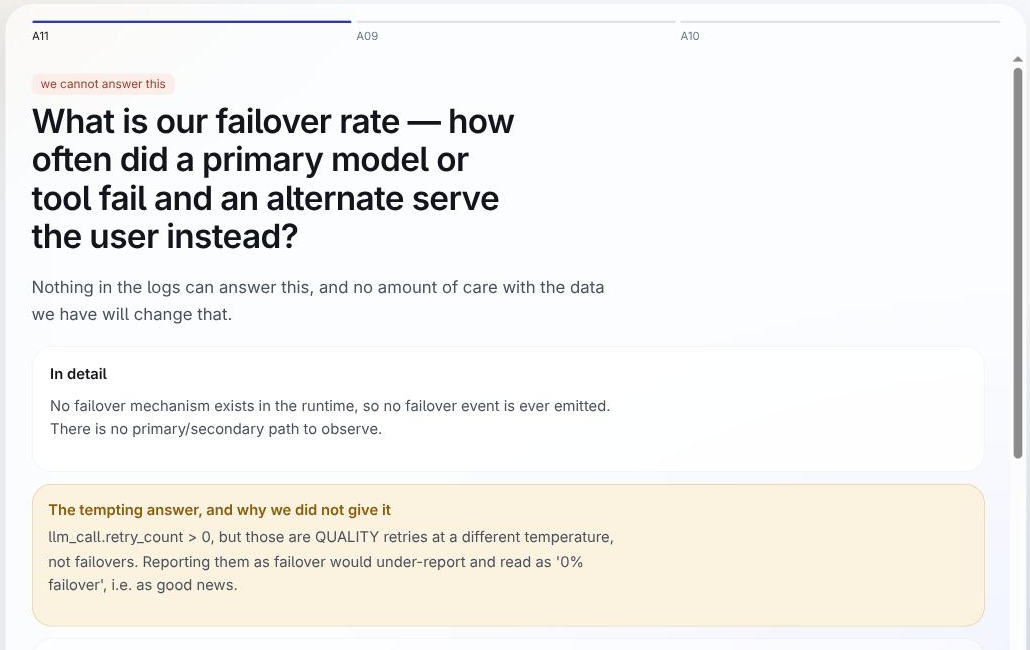
\includegraphics[width=0.99\columnwidth]{figures/operator_refusal.png}
    \caption{The A11 refusal. The proxy is shown and rejected in the same
    breath, because reporting retries as failover would read as
    ``0\,\% failover'' -- false good news.}
    \label{fig:refusal}
\end{figure}

% =========================================================
% 17. FAILURE CASES AND LIMITATIONS
% =========================================================

\section{Failure Cases and Limitations}

\subsection{Known Failure Cases}

\begin{itemize}
    \item A fault planted in the \emph{final} week has under two weeks of
    after-data for onset detection; mitigated because the release gate itself
    needs before/after windows, so extreme-edge planting is unlikely.
    \item The judge-boundary dismissal assumes $\geq2$ tenants (a global rubric
    change affects all of them); it generalises upward, not to a single-tenant
    deployment.
    \item The \texttt{unknown} open-world net is deliberately conservative: it
    requires a two-week, cohort-noise-clearing drop with a real baseline, so it
    will stay silent on a genuinely novel but subtle fault rather than raise a
    weak alarm.
\end{itemize}

\subsection{Scale Limitations}

At $\sim$100$\times$ scale, \texttt{collect\_steps} materializing the step
subsets in memory would need to become a streaming, single-pass aggregation;
the replay budget (40 runs) and the human-review burden, not the analysis
arithmetic, become the binding constraints. The session-grain aggregation and
detection are already single-pass-friendly.

% =========================================================
% 18. ASSUMPTIONS AND TRANSPARENCY
% =========================================================

\section{Assumptions and Transparency}
\label{sec:transparency}

\textbf{Real:} the full Detect$\rightarrow$Diagnose$\rightarrow$Prescribe%
$\rightarrow$Verify loop with the return arrow: the honesty spine, the three
gaps, agnostic anomaly-first detection, deterministic prescriptions, replay
verifications, self-assessment, the hardening harness, and the degradable
preflight. Every analysis number is computed from the corpus, and the core makes
zero LLM/network calls, enforced mechanically. The operator screen is real and
working, including the APPROVE/REJECT gate and its write-back
(\S\ref{sec:screen}). \textbf{Real and run, degradable if unreachable:} the
replay \texttt{verifications} the shipped report carries are a real recorded
run against the organisers' endpoint (\S\ref{sec:verification}), not a
stand-in; if the endpoint is unreachable on a later run the client keeps the
predicted deltas and says so rather than inventing a result.
\textbf{Templated, not generated:} the
plain-language wording on the screen, which is filled from computed numbers by
\texttt{narrate.py} -- no language model writes anything a reader sees.
\textbf{Never written by code:} the human verdicts. The three the shipped
report carries were entered by a person through the screen, the same write
path an operator on the sealed run would use, never by the engine and never
by hand-editing the JSON. \textbf{Simulated:} none. No mocks, no fabricated
numbers, no model in the loop.

\medskip
\noindent\textbf{Disclosure -- what the sealed sweep proves, and what it does
not.} The 80-layout sweep was generated with \emph{our own} passphrases through
the kit's own generator. We never had the organisers' secret and never built
or possessed a sealed kit or its answer key; the organiser-only \texttt{make
sealed} target was never run, and the deliverable path reads no answer key. The
kit's README rests day-6 integrity on the property we left intact:
\emph{``the sealed layout is derived from a passphrase\ldots\ nobody can
regenerate it from this repo alone.''} Our passphrases produce \emph{different}
layouts from the sealed one, so the honest claim is narrow: \textbf{the engine
is robust across this generator's layout \emph{space} -- a distribution, not a
proven claim about an arbitrary real-world deployment or about the organisers'
specific instance.} We state this rather than let the number imply more.

\medskip
\noindent\textbf{The two unbreakable rules hold.} \emph{Rule~1} -- no model is
ever asked for a fact the logs record; every number is computed, and the
analysis core is provably network- and model-free. \emph{Rule~2} -- no metric
definition, judge version, or reviewed ``good'' set was changed to improve a
number; all hardening is to \emph{detection} -- where the engine looks and what
it compares against -- which is the agent, not the yardstick.

% =========================================================
% 19. REPRODUCIBILITY
% =========================================================

\section{Reproducibility}

\subsection{Execution Procedure}

\begin{enumerate}
    \item Python 3.9+; no installs (standard library only).
    \item Place the kit at \texttt{nexus-loop-day1/kit/}.
    \item Run:\\
    {\footnotesize\texttt{python3 -m engine.cli --kit <kit>\\
    \phantom{xx}--team solo --out loop-report.json}}
    \item The report is written and validated against the schema.
    \item Sealed evidence:
    {\footnotesize\texttt{python3 engine/stress\_sealed.py --n 80}}
    (in-memory, from a passphrase; scores each with the organisers'
    \texttt{score.py}).
    \item Launch the operator screen against the report:
    {\footnotesize\texttt{python3 run.py}} --- builds the report if absent,
    serves the screen, and prints what each recorded decision changed in the
    file (\S\ref{sec:screen}).
\end{enumerate}

\subsection{Generated Artifacts}

The submission contains \texttt{loop-report.json}, the complete engine source,
the operator screen, and the run-book. The report is generated by the system
without manual edits.

% =========================================================
% 20. CONCLUSION
% =========================================================

\section*{Conclusion}

We presented \textbf{Nexus Loop}, an autonomous improvement loop that connects
detection, diagnosis, prescription, verification, and human decision-making
into a single workflow. On the practice corpus it identifies \textbf{3} genuine
problems, correctly dismisses \textbf{3} look-alikes, reports \textbf{3}
measurement gaps, and verifies \textbf{3} proposed fixes, scoring
\textbf{55.0\,/\,55}; across 80 sealed-shaped corpora it averages
\textbf{55.00\,/\,55}, the number that actually predicts the sealed run. The
contribution is the \emph{traceable} loop itself: every number has a defined
provenance, every diagnosis is backed by evidence, proposed changes are
verified, and the final action stays in human hands.

% =========================================================
% REFERENCES
% =========================================================

\begin{thebibliography}{9}

\bibitem{YellowAI}
Yellow.ai,
\textit{Nexus Loop -- TECHQUEST Problem Statement Series},
Product Development \& Agentic AI.

\bibitem{Kit}
Yellow.ai,
\textit{Nexus Loop Kit, Schema, Examples and Replay Service},
Provided Challenge Resources.

\end{thebibliography}

\end{document}
